\documentclass[10pt,pdf,hyperref={unicode}]{beamer}

\usepackage{graphicx}
\graphicspath{{./figs/}}

\mode<presentation> {
	\usetheme{Warsaw}
%	\usetheme{chpc}
	  
	\setbeamercovered{transparent}
  % or whatever (possibly just delete it)
}

\usepackage[english]{babel}
%\usepackage[utf8x]{inputenc}

%\usepackage{amsmath}
\usepackage{bm}
\usepackage{tikz}
\usepackage{pgfplots}

\title[] % (optional, use only with long paper titles)
{Automatic Time Step Selection for Numerical Solution of Neutron Diffusion Problems}

%\subtitle
%{Include Only If Paper Has a Subtitle}

\author[] % (optional, use only with lots of authors)
{Aleksandr Avvakumov \inst{1} \and Valery Strizhov \inst{2} \\ 
\and Petr Vabishchevich \inst{2,3} \and \underline{Aleksandr Vasilev \inst{3}}}
% - Give the names in the same order as the appear in the paper.
% - Use the \inst{?} command only if the authors have different
%   affiliation.

\institute[Universities of Somewhere and Elsewhere] % (optional, but mostly needed)
{
\inst{1} National Research Center "Kurchatov Institute", Moscow, Russia
\\
\inst{2} Nuclear Safety Institute, Russian Academy of Sciences, Moscow, Russia
\\ 
\inst{3} North-Eastern Federal University, Yakutsk, Russia
}

% - Use the \inst command only if there are several affiliations.
% - Keep it simple, no one is interested in your street address.

\date[May 25-27, 2017] % (optional, should be abbreviation of conference name)
{7th FDM:T\&A, June 11-16, 2018 Lozenetz}
% - Either use conference name or its abbreviation.
% - Not really informative to the audience, more for people (including
%   yourself) who are reading the slides online

\subject{Theoretical Computer Science}
% This is only inserted into the PDF information catalog. Can be left
% out. 

% ����� � ���������
\graphicspath{{./figs/}}
\newcommand{\grad}{\mathop{\rm grad}\nolimits}
\renewcommand{\div}{\mathop{\rm div}\nolimits}
\newcommand{\const}{\mathop{\rm const}\nolimits}

\begin{document}

\begin{frame}
  \titlepage
\end{frame}

%{
%  \begin{frame}<beamer>
%    \tableofcontents
%  \end{frame}
%}

\section{Introduction}
\begin{frame}{Introduction}
\end{frame}

\section{Problem description}
\subsection{Parabolic equation}
\begin{frame}{Problem description}
Consider second-order parabolic equation
\[
   \frac{\partial u}{\partial t} 
   - \sum_{\alpha =1}^{m}
   \frac{\partial }{\partial x_\alpha} 
   \left ( k({\bm x},t)  \frac{\partial u}{\partial x_\alpha} \right ) + s({\bm x},t) u = f({\bm x},t),
   \quad {\bm x}\in \Omega,
   \quad 0 < t \leq  T,
\]
where
$\underline{k} \leq k({\bm x}) \leq  \overline{k}, \ {\bm x} \in \Omega, \ \underline{k} > 0$.
\vfill

\visible<2,3>{
Boundary condition
\[
   u({\bm x},t) = g({\bm x},t),
   \quad {\bm x}\in \partial \Omega,
   \quad 0 < t \leq  T.
\]
}

\visible<3>{
Initial condition
\[
   u({\bm x},0) = u^0({\bm x}),
   \quad {\bm x}\in \Omega.
\]
}
\end{frame}

\subsection{Operator notation}
\begin{frame}{Operator notation}
Cauchy problem
\[
  \frac{du}{dt} + A(t) u = f(t),
  \quad 0 < t \leq T,
\]
with initial condition
\[
   u(0) = u_0.
\]
\vfill

\visible<2>{
Assume $A(t) \geq 0$ in $H$ then
\[
  \|u(t)\| \leq \|u_0\| + \int_{0}^{t} \|f(\theta) \| d \theta .
\]
}
\end{frame}

\subsection{Solution evaluation}
\begin{frame}{Solution evaluation}
Introduce irregular time grid
\[
 t^0=0, \quad t^{n+1} = t^n + \tau^{n+1},
 \quad n = 0,1, ..., N-1,
 \quad t^n = T .   
\] 
\visible<2,3,4>{
Implicit scheme are used
\[
  \frac{y^{n+1} - y^{n}}{\tau^{n+1}} + A^{n+1} y^{n+1} = f^{n+1},
  \quad n = 0,1, ..., N-1,
\]
and initial condition $y^0 = u^0.$
}

\vfill

\visible<3,4>{
Layerwise estimate ($A^{n+1} \geq 0$)
\[
 \|y^{n+1}\| \leq \|y^{n}\| + \tau^{n+1} \|f^{n+1}\|.
\]
}

\visible<4>{
Difference estimate
\[
 \|y^{n+1}\| \leq \|u^{0}\| + \sum_{k=0}^{n} \tau^{k+1} \|f^{k+1}\|.
\]
}
\end{frame}

\subsection{Solution error}
\begin{frame}{Solution error}
For $z^n = y^n - u^n$:
\[
  \frac{z^{n+1} - z^{n}}{\tau^{n+1}} + A^{n+1} z^{n+1} = \psi^{n+1},
  \quad n = 0,1, ..., N-1,  
\] 
\[
 z^0 = 0.
\] 

\visible<2,3,4>{
Approximation error
\[
 \psi^{n+1} = f^{n+1} -
 \frac{u^{n+1} - u^{n}}{\tau^{n+1}} - A^{n+1} u^{n+1} . 
\]
}

\visible<3,4>{
Layerwise estimate
\[
  \|z^{n+1}\| \leq \sum_{k=0}^{n} \tau^{k+1} \|\psi^{k+1}\| .
\]
}

\visible<4>{
Difference estimate
\[
 \|z^{n+1}\| \leq \delta t^{n+1}.
\] 
}
\end{frame}

\subsection{Algorithm}
\begin{frame}{Time step selection algorithm}
\begin{enumerate}
\item 
Predictable time step: $\widetilde{\tau}^{n+1} = \gamma \tau^n$ (eg $\gamma=1.25$)

\visible<2,3,4,5>{
\item Predictive solution $\widetilde{y}^{n+1}$: an explicit scheme, $\widetilde{t}^{n+1} = t^n + \widetilde{\tau}^{n+1}$
}

\visible<3,4,5>{
\item Estimation of approximation error: by found $\widetilde{y}^{n+1}$ from an implicit scheme
}

\visible<4,5>{
\item Step selection $\tau^{n+1}$: $\ \|\psi^{n+1}\| \approx \delta$
}

\visible<5>{
\item Solution on a new time layer $y^{n+1}$: an implicit scheme, $t^{n+1}=t^n + \tau^{n+1}$
}
\end{enumerate}
\end{frame}

\section{Time step estimate}
\subsection{Neutron diffusion equation}
\begin{frame}{Neutron diffusion equation}
One group diffusion approximation with one group delayed neutron sources
\[
\begin{split}
 \frac{1}{v} \frac{\partial \phi}{\partial t} -  \nabla \cdot D \nabla \phi + \Sigma_{a} \phi &=   \ (1-\beta) \nu \Sigma_{f} \phi + \lambda c, \\
\frac{\partial c}{\partial t} + \lambda c &= \beta \nu \Sigma_{f} \phi.
\end{split}
\]
Boundary condition
\[
 D\frac{\partial \phi}{\partial n} + \gamma \phi = 0.
\]
Initial conditions
\[
 \phi(0) = \phi^0,  \,
 c(0) = c^0.
\]
\end{frame}

\subsection{Calculated formulas}
\begin{frame}{Calculated formulas}

The approximation error
\[
\begin{split}
\bm{\widetilde{\psi}^{n+1}} &= (A^{n+1} - A^n)\bm{\varphi^n} + {A}^{n+1}(\bm{\widetilde{\varphi}^{n+1}} - \bm{\varphi^n}) \\
&= \widetilde{\tau}^{n+1} \left( \frac{A^{n+1} - A^n}{\widetilde{\tau}^{n+1}} \bm{\varphi^n} + A^{n+1} \frac{\bm{\widetilde{\varphi}^{n+1}} - \bm{\varphi^n}}{\widetilde{\tau}^{n+1}} \right),
\end{split}
\]
Error $\widetilde{\bm\psi}^{n+1}$ compare with $\widetilde{\tau}^{n+1}$, and $\bm\psi^{n+1}$ with step $\tau^{n+1}$:
\[
  \bar{\tau}^{n+1} = \gamma_{n+1} \tau^n,
  \quad \gamma_{n+1} = \frac{\delta}{\|\widetilde{\bm\psi}^{n+1}\|}  \gamma .
\]
Where
$\bm{\varphi^n} = \{\varphi^n, s^n\}$, $\bm{\psi^{n+1}} = \{\psi^{n+1}_1, \psi^{n+1}_2\}$, $\bm{\widetilde{\psi}^{n+1} }= \{\widetilde{\psi}^{n+1}_1, \widetilde{\psi}^{n+1}_2\}$,
\[
\begin{split}
A &= \begin{pmatrix}
  - \nabla \cdot D \nabla  + \Sigma_{a}  - (1-\beta) \nu \Sigma_{f} - \lambda & 0  \\
  0  & \lambda - \beta\nu\Sigma_f   \\
 \end{pmatrix}.
\end{split} 
\]
\end{frame}

\begin{frame}
The needed time step
\[
 \tau^{n+1} \leq \bar{\tau}^{n+1},
 \quad  \tau^{n+1} \leq \widetilde{\tau}^{n+1},
 \quad
  \tau^{n+1} = \max \big \{\tau^0, \min \{\gamma_{n+1}, \gamma \} \tau^n \big \}. 
\] 
The approximation error has the first order in time
\[
\bm{\widetilde{\psi}^{n+1}} = \mathcal{O} (\widetilde{\tau}_{n+1}).
\]
In view of this, we set 
\[
 \|\bm{\widetilde{\psi}^{n+1}} \| \leq \| (A^{n+1} - A^n) \bm{\varphi^n} +
 A^{n+1} (\bm{\widetilde{\varphi}^{n+1}} - \bm{\varphi^n}) \| .
\]
Calculated formula for time step
\[
  \gamma_{n+1} = \frac{\delta}{ \| (A^{n+1} - A^n) \bm{\varphi^n}  +
  A^{n+1} (\bm{\widetilde{\varphi}^{n+1}} - \bm{\varphi^n}) \| } \gamma .
\]
\end{frame}

\section{Benchmark}
\subsection{General description}
\begin{frame}{IAEA-2D benchmark}
	\begin{columns}[]
		\column{0.5\textwidth}
			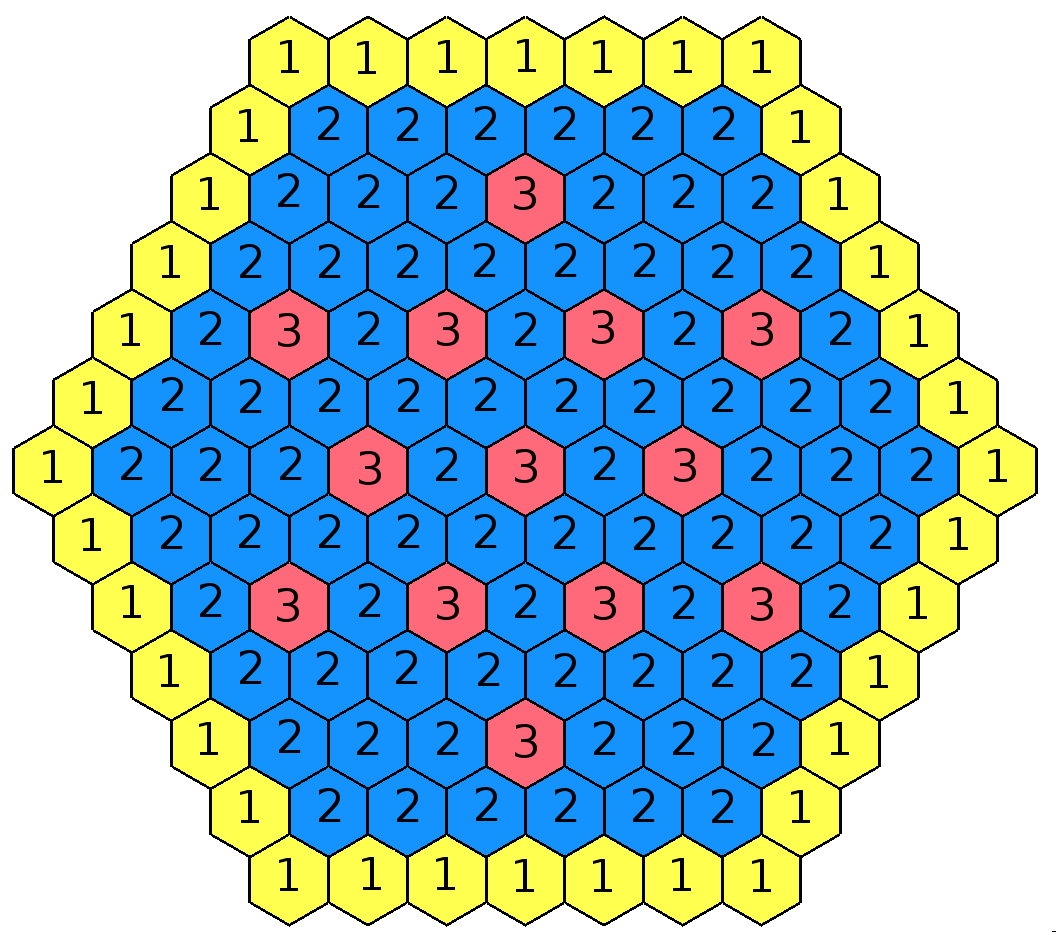
\includegraphics[width=1\linewidth]{ts_iaea/1.png}
		\column{0.5\textwidth}
			\begin{itemize}
				\item One group of instantaneous neutrons
				\item One group of delayed neutrons
				\item Modeling effect of immersion or extraction of control rods
			\end{itemize}
	\end{columns}
\end{frame}

\subsection{Computational results}
\begin{frame}{Nuclear power}
\begin{center}
    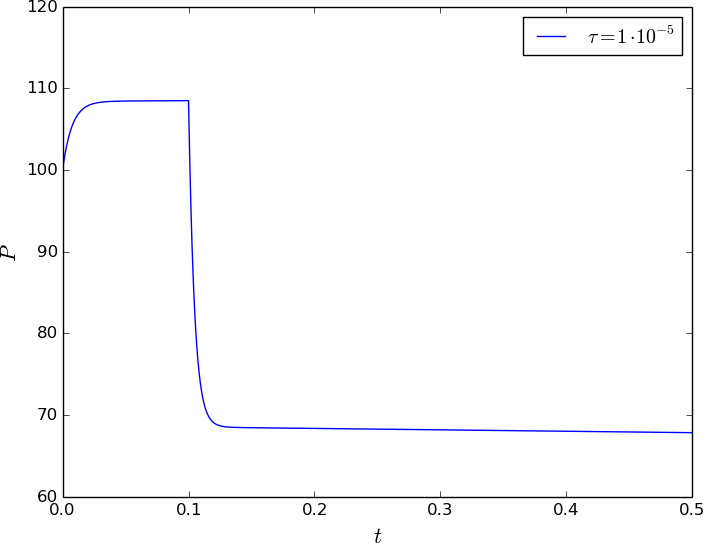
\includegraphics[width=0.49\linewidth] {ts_iaea/power_down.png}
    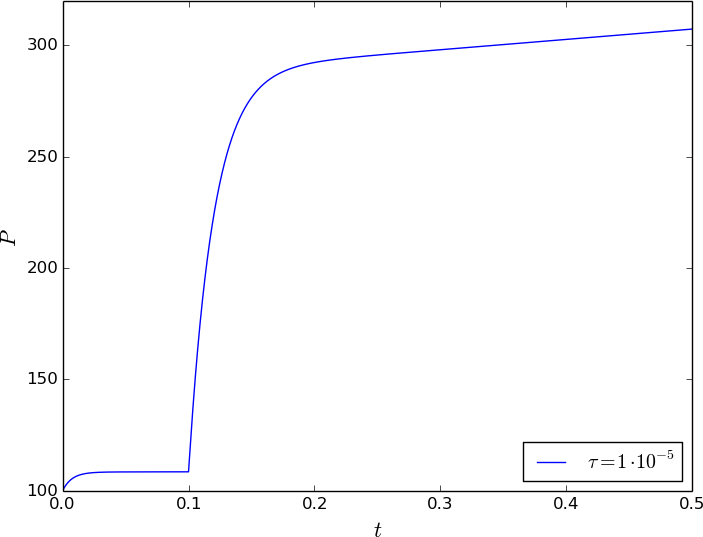
\includegraphics[width=0.49\linewidth] {ts_iaea/power_up.png}
    \\
	Nuclear power for immersion (left) and extraction (right).
    \[
    P(t)=a \sum_{g=1}^G\int_{\Omega}\Sigma_{fg}\phi_g d\bm x,
    \]
    where $a$ -- normalization factor.
\end{center}
\end{frame}

\begin{frame}{Error}
\begin{center}
    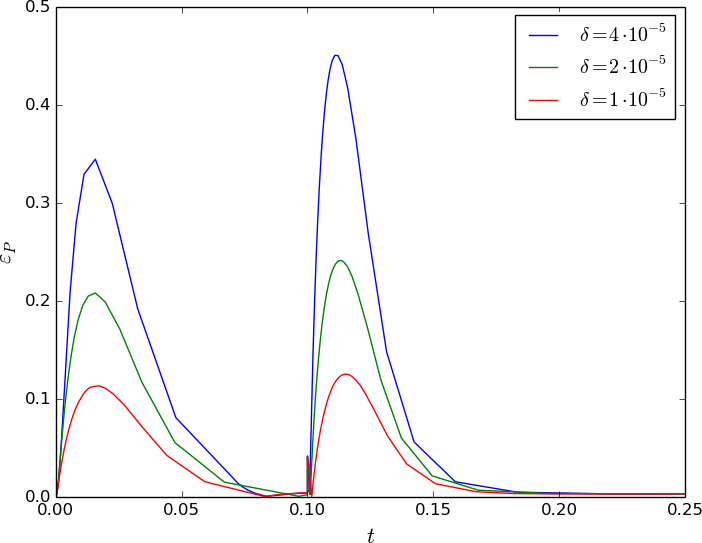
\includegraphics[width=0.49\linewidth] {ts_iaea/delta_down.png}
    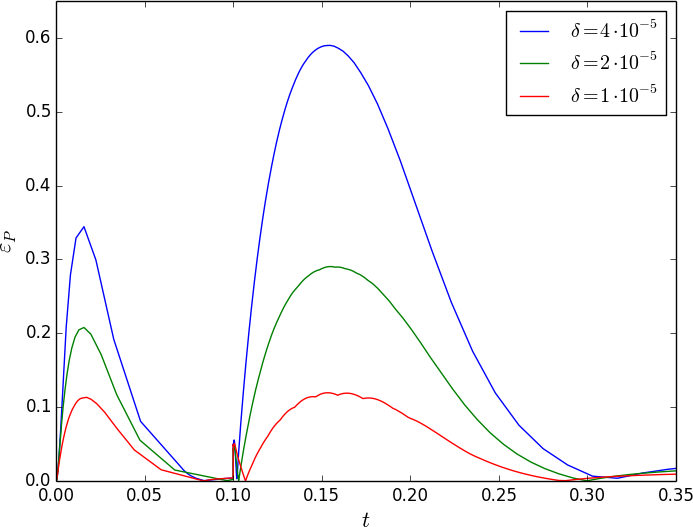
\includegraphics[width=0.49\linewidth] {ts_iaea/delta_up.png}
    \\
	Error for immersion (left) and extraction (right).
     \[
     \epsilon_P(t) = | P_{ref} - P|,
     \]
     where $P_{ref}$ -- reference solution.
\end{center}
\end{frame}

\subsection{Software}
\begin{frame}{Software}
\begin{center}
	{
\includegraphics[width=0.4\linewidth] {gmsh.png}}
    \hfill
    \visible<2,3,4>{
\includegraphics[width=0.49\linewidth] {slepc.png}}
    \vfill
	\visible<3,4>{
\includegraphics[width=0.49\linewidth] {fenics.png}}
    \hfill
    \visible<4>{
\includegraphics[width=0.49\linewidth] {python.png}}
\end{center}
\end{frame}

\begin{frame}{Time step}
\begin{center}
	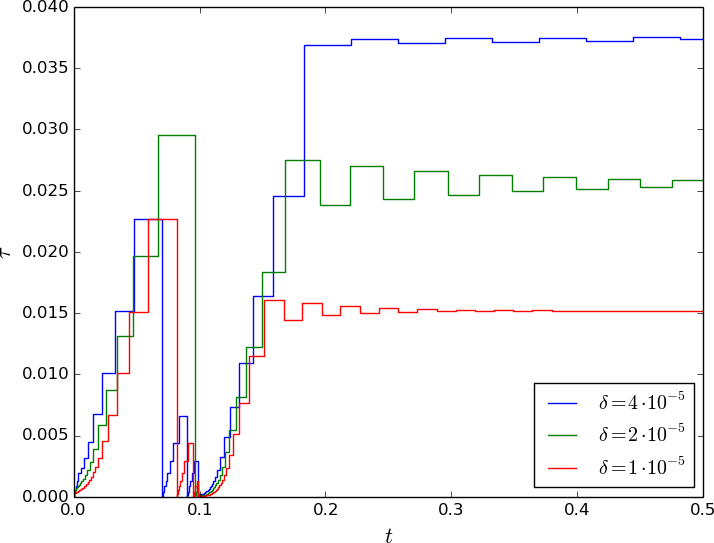
\includegraphics[width=0.49\linewidth] {ts_iaea/step_down.png}
    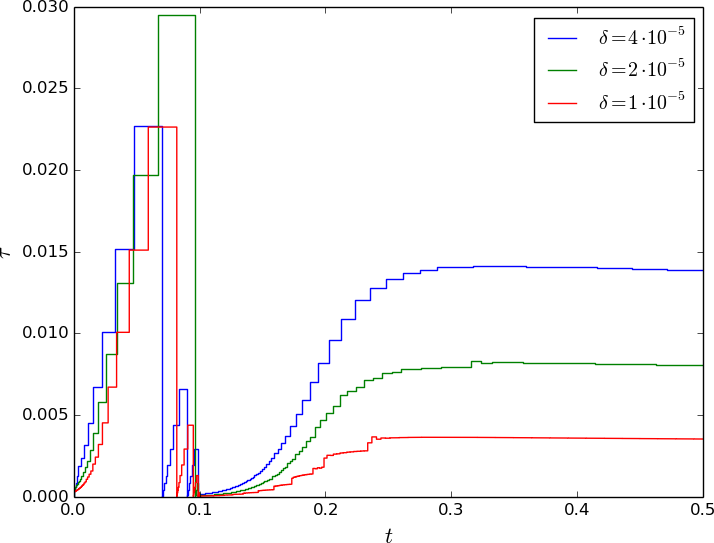
\includegraphics[width=0.49\linewidth] {ts_iaea/step_up.png}
    \\
	Time steps for immersion (left) and extraction (right).
\end{center}
\end{frame}

\begin{frame}{Counting time and number of steps}
\begin{table}[htp]
\begin{center}
\begin{tabular}{ccrrcrr}
&\multicolumn{3}{c}{immersion} & \multicolumn{3}{c}{extraction}\\
\hline
$\delta$ & max($\epsilon_P$) & $n$ & $t$, sec & max($\epsilon_P$)  & $n$ & $t$, sec \\
\hline
$4\cdot 10^{-5}$ & 0.450 & 136 & 16 & 0.590 & 241 & 35 \\
$2\cdot 10^{-5}$ & 0.241 & 159 & 20 & 0.290 & 373 & 62 \\
$1\cdot 10^{-5}$ & 0.125 & 270 & 37 & 0.120 & 773 & 145 \\
\hline
\end{tabular}
\end{center}
\end{table}
\vspace{5mm}
Reference solution: fixed time step $10^{-5}$, number of steps -- 50000,  counting time -- 2130 sec. 
\vfill
\visible<2>{
\begin{center}
\large
Thank you for your attention!
\end{center}
}

\end{frame}


\end{document}
